\documentclass{article}
\usepackage{graphicx}

\title{Implementation}
\begin{document}
    \maketitle

    A system was developed to perform two way conversion from natural language to actions, and from actions to natural language.

    \section{Natural language to Actions}
    \begin{figure}
        \begin{center}        
            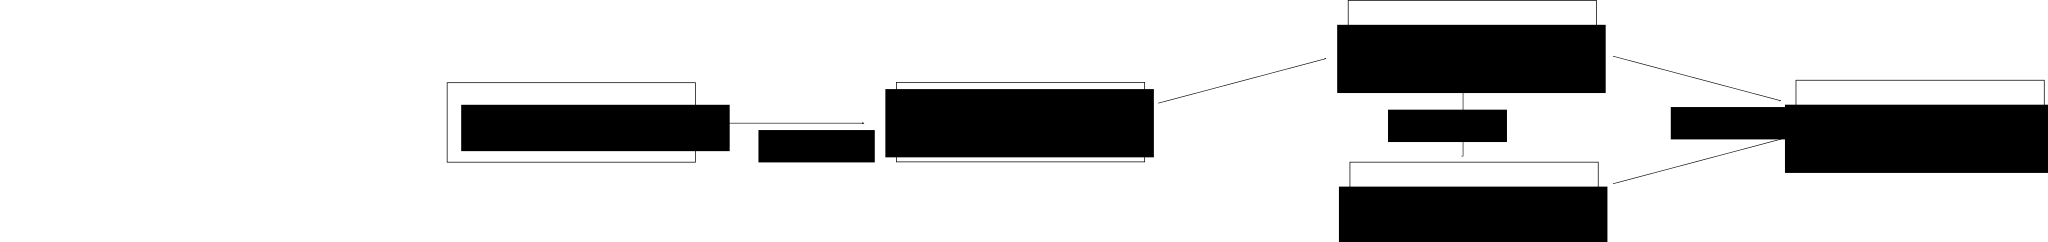
\includegraphics[width=300pt]{diagrams/verb-to-action-workflow.png}
        \end{center}
        \caption{The workflow for parsing an event expressed in natural lanuage into it's physical representation}
    \end{figure}

    The first step is parsing a natural language event into a predicate-argument structure relating subject and object. Each verb sense will have a definition in terms of conceptual dependencies- which CD primitive it corresponds to, which physical attribute it affects (e.g.~the `eject' verb indicates the object has been removed from inside the subject, meaning an `inside\_subject' attribute is assigned to that verb).

    Each verb definition will have a CD primitive associated with it- each of these primitives will have it's own properties such as the attribute it affects, and any constraints on the subject/ object type. The verb definition is then merged with the primitive definition (there should be no contradictory fields).
    
    \section{Actions to Natural Language}
    \begin{figure}
        \begin{center}        
            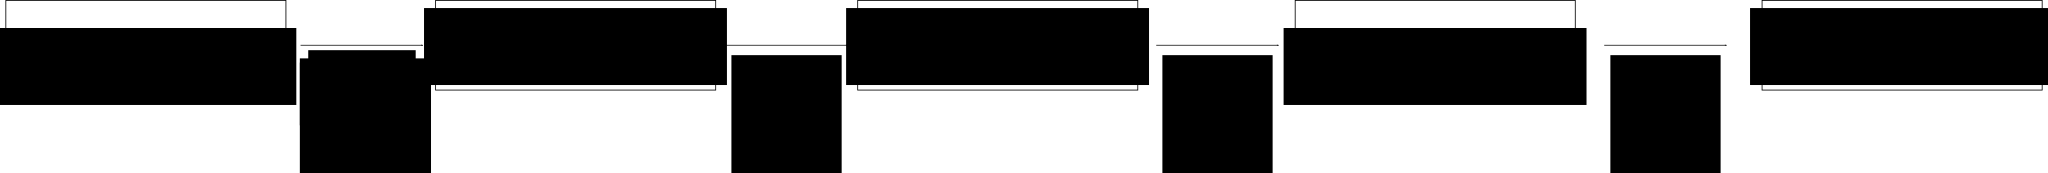
\includegraphics[width=300pt]{diagrams/action-to-verb-workflow.png}
        \end{center}
        \caption{The workflow for parsing an event expressed in natural lanuage into it's physical representation}
    \end{figure}
\end{document}